\chapter{Literatuurstudie}
\label{ch:literatuurstudie}

% Tip: Begin elk hoofdstuk met een paragraaf inleiding die beschrijft hoe
% dit hoofdstuk past binnen het geheel van de bachelorproef. Geef in het
% bijzonder aan wat de link is met het vorige en volgende hoofdstuk.

Deze literatuurstudie zal samen met de lijst van termen uit hoofdstuk \ref{ch:termen} de nodige achtergrondinformatie bieden om de volgende delen van de paper te begrijpen. Er zal verwezen worden naar meerdere papers van andere instellingen zodanig dat u zich verder kan inlezen waar gewenst.

% Pas na deze inleidende paragraaf komt de eerste sectiehoofding.


%Dit hoofdstuk bevat je literatuurstudie. De inhoud gaat verder op de inleiding, maar zal het onderwerp van de bachelorproef *diepgaand* uitspitten. De bedoeling is dat de lezer na lezing van dit hoofdstuk helemaal op de hoogte is van de huidige stand van zaken (state-of-the-art) in het onderzoeksdomein. Iemand die niet vertrouwd is met het onderwerp, weet nu voldoende om de rest van het verhaal te kunnen volgen, zonder dat die er nog andere informatie moet over opzoeken \autocite{Pollefliet2011}.

%Je verwijst bij elke bewering die je doet, vakterm die je introduceert, enz. naar je bronnen. In \LaTeX{} kan dat met het commando \texttt{$\backslash${textcite\{\}}} of \texttt{$\backslash${autocite\{\}}}. Als argument van het commando geef je de ``sleutel'' van een ``record'' in een bibliografische databank in het Bib\LaTeX{}-formaat (een tekstbestand). Als je expliciet naar de auteur verwijst in de zin, gebruik je \texttt{$\backslash${}textcite\{\}}.
%Soms wil je de auteur niet expliciet vernoemen, dan gebruik je \texttt{$\backslash${}autocite\{\}}. In de volgende paragraaf een voorbeeld van elk.


%\textcite{Knuth1998} schreef een van de standaardwerken over sorteer- en zoekcompressie-algoritmen. Experten zijn het erover eens dat cloud computing een interessante opportuniteit vormen, zowel voor gebruikers als voor dienstverleners op vlak van informatietechnologie~\autocite{Creeger2009}.

\section{Bestandsgrootte en dataopslag}
\label{sec:bestandsgrootte-dataopslag}
Zoals in de definitie van \gls{datacompressie} besproken is, bestaat \gls{datacompressie} uit het digitaal opslaan van een bestand met zo weinig mogelijk \glspl{bit}.

\Gls{bit} staat kort voor binary digit. Een bit wordt beschouwd als de kleinste data eenheid voor dataopslag. Een bit kan twee waarden aannemen, deze worden voorgesteld door 1 of 0 (binair talstelsel) maar kunnen ook geïnterpreteerd worden als aan of uit, ja of nee…

\subsection{Voorvoegsels voor het uitdrukken van bestandsgrootte}
\label{sec:bestandsgrootte-dataopslag-voorvoegsels}

Bestandsgroottes worden meestal uitgedrukt in bytes (8 bits), al dan niet met voorvoegsel dat een veelvoud voorstelt. Deze voorvoegsels en het door elkaar gebruik van de \gls{si-voorstelling-bestandsgrootte} en \gls{binaire-voorstelling-bestandsgrootte} kan voor enige verwarring zorgen. Denk hierbij aan het fenomeen dat harde schijven die geadverteerd zijn als 1TB (\gls{si-voorstelling-bestandsgrootte}) overeen komt met 931GiB (\gls{binaire-voorstelling-bestandsgrootte}) op de meeste besturingssystemen. Doorheen deze paper zal de \gls{si-voorstelling-bestandsgrootte} gebruikt worden.

\subsubsection{SI voorstelling}
\label{sec:bestandsgrootte-dataopslag-voorvoegsels-si}

De \gls{si-voorstelling-bestandsgrootte} gebruikt als basis 1000 wat overeen komt met $ 10^{3} $. SI staat voor International System of Units en beschrijft. Het wordt beschouwd als een moderne vorm op het metrisch stelsel. SI beschrijft onder IEC 60027 het gebruik van bepaalde voorvoegsels voor het uitdrukken van machten op 10. (\cite{iec60027}) Een conversietabel is hieronder raadpleegbaar. 

\FloatBarrier
\begin{table}[h]
	\begin{tabular}{lll}
		Voorvoegsel & symbool & waarde \\
		kilo & Ki & $ 10^{3} = 1000^{1} $  = 1 000 \\
		mega & Mi & $ 10^{6} = 1000^{2} $  = 1 000 000 \\
		giga & Gi & $ 10^{9} = 1000^{3} $  = 1 000 000 000
	\end{tabular}
\end{table}
\FloatBarrier

\subsubsection{binaire voorstelling}
\label{sec:bestandsgrootte-dataopslag-voorvoegsels-binair}

De \gls{binaire-voorstelling-bestandsgrootte} gebruikt als basis 1024 wat overeen komt met $ 2^{10} $. Deze voorstelling is een standaardisatie opgelegd door \gls{ieee} 1541-2002 (\cite{ieee15412002}). Een conversietabel is hieronder raadpleegbaar.

\FloatBarrier
\begin{table}[h]
	\begin{tabular}{lll}
		Voorvoegsel & symbool & waarde \\
		kibi & Ki & $ 2^{10} = 1024^{1} $  = 1 024 \\
		mebi & Mi & $ 2^{20} = 1024^{2} $ = 1048 576 \\
		gibi & Gi & $ 2^{30} = 1024^{3} $ = 1 073 741 824
	\end{tabular}
\end{table}
\FloatBarrier

\subsubsection{clustergrootte}
\label{sec:bestandsgrootte-dataopslag-clustergrootte}

Een andere belangrijke term bij dataopslag is de \gls{clustergrootte}. Data moet namelijk bijgehouden worden in één of meerdere \glspl{cluster} op een opslagmedium zodat naar deze \glspl{cluster} kan verwezen worden voor het lezen van de data. 

Aangezien alle data steeds minstens in één \gls{cluster} staat en twee verschillende databestanden nooit een \gls{cluster} kunnen delen kan dit voor opslagruimteverlies zorgen. 

Neem bijvoorbeeld een \gls{clustergrootte} van 4096 \glspl{byte}, een vaak voorkomende \gls{clustergrootte}. Als in deze situatie een bestand van 2000 \glspl{byte} groot zou opgeslagen worden, zijn de overige 2096 \glspl{byte} aan opslagcapaciteit op die schijf verloren. Een bestand van 4097 \glspl{byte} zou twee \glspl{cluster} in beslag nemen waardoor 4095 \glspl{byte} verloren gaan. 

Dit speelt vooral een rol wanneer \gls{datacompressie} gebruikt wordt voor het besparen van opslagruimte op een opslagmedium. Een gecomprimeerd bestand met een kleinere bestandsgrootte dat dezelfde hoeveelheid \glspl{clustergrootte} nodig heeft op het medium zal dus niet voor plaats besparing zorgen op dat opslagmedium. 

Theoretisch gezien zal er wel een verbetering te zien zijn in \glspl{leestijd} en de gebruikte \gls{bandbreedte} bij een bestandsoverdracht omdat de effectieve bestandsgrootte kleiner is. 

Er zijn tal van reden waarom een andere \gls{clustergrootte} aangeraden is, een recente discussie is terug te vinden in een blogpost van Microsoft\urlcite{microsoftblogcluster}

\section{Ontstaan datacompressie en primitieve technieken}
\label{sec:ontstaan-datacompressie-primitieve-technieken}
\subsection{Eerste vorm van datacompressie}
\label{sec:ontstaan-datacompressie-primitieve-technieken-eerste-vorm}
Vele onderzoekers zijn het erover eens dat \gls{datacompressie} dateert van voor de uitvinding van de computer. Vele onderzoekers zijn het er over eens dat morsecode de eerste vorm was van \gls{datacompressie}. Morsecode is uitgevonden in 1832 door Samuel F.B. Morse en wordt aanzien als eerste vorm van datacompressie doordat veel voorkomende letters een kortere audiotoon kregen dan minder gebruikte letters. (\cite{morsecode})

\subsection{Ontwikkeling datacompressie binnen IT}
\label{sec:ontstaan-datacompressie-primitieve-technieken-binnen-it}
Bij de prille opkomst van mainframe eind de jaren 40 en begin de jaren 50 zijn twee belangrijke doorbraken binnen \gls{datacompressie} gemaakt. Beiden maken gebruik van \gls{prefix-code}. De originele uitvinder van dit soort compressie was Shannon Claude dat Shannon coding uitvond, een proof of concept voor zijn artikel \citetitle{shannon1948} (\cite{shannon1948}). In diezelfde periode werd ook Shannon-Fano coding voorgesteld, een project samen met Robert Fano dat verschillende \glspl{use-case} had. Geen van beide technieken waren echter optimaal aangezien de \glspl{compressie-algoritme} niet gegarandeerd de korst mogelijke prefix codes gaven. 

\Gls{huffman-coding}, voorgesteld in  \citetitle{huffman} (\cite{huffman}) was een optimale variant op deze techniek. Dit is een \gls{compressie-algoritme} door David Huffman gemaakt als academie opdracht dat bijna 70 jaar na publicatie nog steeds de basis legt voor vele \gls{lossless} \gls{datacompressie} \glspl{compressie-algoritme}. Deze soort \glspl{compressie-algoritme} worden \gls{frequency-based} \glspl{compressie-algoritme} genoemd. Het exacte verschil tussen \gls{huffman-coding} en Shannon-Fano coding en meer informatie over deze \glspl{compressie-algoritme} zijn beschreven in \citetitle{lelewer87datacompression} (\cite{lelewer87datacompression}). In deel \ref{sec:primitieve-technieken-voorbeeld-huffman-encoding} wordt een praktisch voorbeeld van \gls{huffman-coding} uitgewerkt. In hoofdstuk  \ref{ch:compressietool} zal onder andere \gls{huffman-coding} gebruikt worden voor het maken van de compressietool.

De jaren 70 en 80 zorgden voor tal van belangrijke doorbraken binnen \gls{datacompressie}. Dit was te weiden aan de opkomst van het internet en de steeds groter wordende bestanden. Ook werd hardware matige compressie (zoals \gls{prefix-code} met vaste \gls{lookup-table} voor tekstbestanden) steeds meer vervangen door dynamische compressie (codegewijs). 

Deze eerste softwareoplossingen waren veelal implementatie van \gls{huffman-coding}, eventueel met kleine aanpassingen. Eind de jaren 70 waren de eerste Lempel-Ziv \gls{compressie-algoritme} uitgevonden: LZ77 en LZ78. Dit zijn de grondleggers van \gls{dictionary-coding}. Een veelgebruikte variant van LZ798 is LZW (1984). Net zoals \gls{huffman-coding} de basis legde voor vele van de eerste softwareoplossingen zorgde de grondleggers van \gls{dictionary-coding} voor vele nieuwe softwareoplossingen. De doorgroei van deze \glspl{compressie-algoritme} is zichtbaar in figuur \ref{fig:lossles-datacompressie-overzicht}.

\begin{figure}
	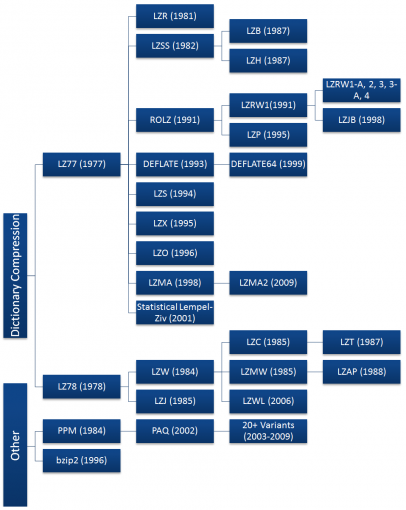
\includegraphics{img/literatuurstudie/lossles_datacompressie_overzicht.png}
	\caption{Lossless datacompressie overzicht (\cite{ethwcompressionhistory})}
	\label{fig:lossles-datacompressie-overzicht}
\end{figure}

Het grootste verschil tussen \gls{prefix-coding} en \gls{dictionary-coding} zit in de naam zelf. Bij \gls{prefix-coding} wordt elk karakter vervangen door een \gls{prefix-code} terwijl bij \gls{dictionary-coding} een reeks van karakters vervangen kunnen worden door één enkele \gls{prefix-code}.  

Eind de jaren 80 en begin de jaren 90, door de digitalisering van afbeeldingen en muziek, begonnen \gls{lossy} \glspl{compressie-algoritme} steeds meer op te komen. Het verschil tussen \gls{lossless} en \gls{lossy} \glspl{compressie-algoritme} wordt in deel \ref{sec:ontstaan-datacompressie-lossless-lossy} verder besproken.


\subsection{Primitieve technieken: een voorbeeld}
\label{sec:primitieve-technieken-voorbeeld}
TODO

\subsubsection{Situering}
\label{sec:primitieve-technieken-voorbeeld-situering}
TODO

\subsubsection{ASCII encoding en decoding}
\label{sec:primitieve-technieken-voorbeeld-ascii}
TODO

\paragraph{ASCII Probleemstelling 1: 8 bits per karakter}
\label{par:primitieve-technieken-voorbeeld-ascii-probleem-1}
TODO

\subsubsection{RLE: run length encoding en decoding}
\label{sec:primitieve-technieken-voorbeeld-rle}
TODO

\paragraph{RLE Probleemstelling 1: gecomprimeerd bestand groter dan bron}
\label{par:primitieve-technieken-voorbeeld-rle-probleem-1}
TODO

\subsubsection{Huffman coding}
\label{sec:primitieve-technieken-voorbeeld-huffman-encoding}
TODO

\paragraph{Huffman encoding stap 1: meerdere bomen}
\label{par:primitieve-technieken-voorbeeld-huffman-encoding-1}
TODO

\paragraph{Huffman encoding stap 2: bomen samenvoegen}
\label{par:primitieve-technieken-voorbeeld-huffman-encoding-2}
TODO

\paragraph{stap 3: prefix tabel (optioneel)}
\label{par:primitieve-technieken-voorbeeld-huffman-encoding-3}
TODO

\paragraph{stap 4: encoding}
\label{par:primitieve-technieken-voorbeeld-huffman-encoding-4}
TODO

\paragraph{Huffman decoding}
\label{par:primitieve-technieken-voorbeeld-huffman-decoding}
TODO

\paragraph{Huffman coding Probleemstelling 1: binaire boom niet opgeslagen}
\label{par:primitieve-technieken-voorbeeld-huffman-probleem-1}
TODO

\paragraph{Huffman coding Probleemstelling 2: gecomprimeerd bestand groter dan bron}
\label{par:primitieve-technieken-voorbeeld-huffman-probleem-2}
TODO

\paragraph{Huffman coding Probleemstelling 3: overlappende prefix codes}
\label{par:primitieve-technieken-voorbeeld-huffman-probleem-3}
TODO

\section{Lossless vs lossy datacompressie}
\label{sec:ontstaan-datacompressie-lossless-lossy}
